\documentclass[11pt, a4paper, final]{article}

\usepackage[margin=1in, bottom=1in]{geometry}
\usepackage{amsmath}
\usepackage{graphicx}
\usepackage{amsfonts}
\usepackage{url}
\urlstyle{same}
\usepackage{titling}
\usepackage{lipsum}
\usepackage{setspace}
\usepackage{hyperref}
\usepackage{amsthm}

\newcommand\onlyb[1]{\normalfont{\textbf{#1}}}
\newcommand\noSty[1]{\normalfont{#1}}
\newtheorem{theorem}{Teorema}[section]
\newtheorem{lemma}[theorem]{Lema}
\newtheorem{definition}[theorem]{Definisi}
\newtheorem{proposition}[theorem]{Proposisi}

% Bibliography stuffs i believe
\usepackage[bahasa]{babel}
\usepackage[fixlanguage]{babelbib}

% Bold extra
\usepackage{bold-extra}

% Image floating
\usepackage{float}

% Image subfigure
\usepackage{caption}
\usepackage{subcaption}

% Code highlight
\usepackage[newfloat]{minted}
\usepackage{xcolor} % to access the named colour LightGray
\definecolor{LightGray}{gray}{0.9}

% Pseudocode
\usepackage[ruled,linesnumbered]{algorithm2e}
\renewcommand*{\algorithmcfname}{Algoritma}
\SetKwInput{KwData}{Masukan}
\SetKwInput{KwResult}{Keluaran}

% Separator length in itemize
\usepackage{enumitem}

\begin{document}
% Here goes the title hehehe
\begin{center}
    \Large
    \textbf{Struktur Data Eertree dan Variasinya dalam Menyelesaikan Permasalahan Substring Palindrom\\}
    \vspace{0.2cm}
    \Large
    Hocky Yudhiono – 1906285604\\
    \texttt{hocky.yudhiono@ui.ac.id}\\
    \vspace{0.2cm}
    \large
    Fakultas Ilmu Komputer, Universitas Indonesia\\
\end{center}
\onehalfspacing

\section{Pendahuluan}

Karya ini merupakan hasil studi pustaka dari \textit{\textbf{Eertree: An efficient data structure for processing palindromes in strings}} oleh Rubinchik, M. dan Shur, A. M. pada tahun 2018. Kemiripan observasi dan alur pendekatan permasalahan yang serupa merupakan hasil pemikiran dari penulis \textit{paper} tersebut. Penjelasan, bukti, dan elaborasi ditulis ulang dalam bentuk pemahaman saya.

Palindrom merupakan salah satu bentuk dari sebuah \textit{string}. Sebuah \textit{string} $S$ dengan panjang $n$ disebut palindrom ketika \textit{string} tersebut sama dengan kebalikan dari \textit{string} itu sendiri. Dengan kata lain, berlaku $S=c_1c_2\dots c_n=c_n \dots c_2 c_1$. \textit{Palindromic Tree} atau biasa dikenal dengan Eertree merupakan salah satu struktur data yang ditemukan dan dirilis jurnalnya oleh Mikhail Rubinchik pada tahun 2017. Eertree dapat melakukan berbagai macam operasi terhadap palindrom pada sebuah \textit{string} $S$ dalam kompleksitas waktu $O(n \log |\sigma|)$, untuk $|\sigma|$ merupakan kardinalitas dari himpunan $\sigma$ yang merupakan karakter berbeda yang menyusun $S$. Selanjutnya, kita definisikan pula $S[L, R]$ sebagai \textit{substring} inklusif dari indeks $L$ hingga $R$.

\section{Masalah}

Ada banyak jenis operasi yang dapat dilakukan oleh Eertree. Berikut ialah beberapa permasalahan yang dapat dikerjakan dengan Eertree.

\subsection{Substring Palindrom Berbeda}
\subsubsection{Deskripsi dan Batasan}
Diberikan sebuah \textit{string} $S$ sepanjang $n$, tentukan ada berapa banyak \textit{substring} palindrom tak kosong berbeda yang terdapat untuk setiap \textit{prefix} S, yaitu \textit{substring} $S[1, 1], S[1, 2], S[1, 3],$ $\dots, S[1, n]$. Tanpa kehilangan sifat umum, definisikan batasan-batasan untuk masalah ini ialah sebagai berikut.

\begin{itemize}
  \setlength\itemsep{-0.5em}
  \item $1 \leq n \leq 1\,000\,000$
  \item \textit{String} $S$ hanya terdiri dari huruf latin kecil ($\texttt{a}-\texttt{z}$). Dengan kata lain, $\sigma = [\texttt{a},\texttt{z}]$ dan $|\sigma| = 26$.
\end{itemize}

\subsubsection{Contoh Masukan dan Keluaran}

Algoritma menerima masukan sebuah \textit{string} $S$ sepanjang $n$ dan akan mengembalikan $n$ buah bilangan bulat yang menyatakan banyaknya \textit{substring} palindrom berbeda untuk setiap \textit{prefix} $S[1, i]$ $(1 \leq i \leq n)$. Misalkan masukan merupakan sebuah \textit{string} $S = \texttt{eertree}$. Observasi untuk setiap \textit{prefix} $S[1, i]$ ialah sebagai berikut.

\begin{itemize}
  \setlength\itemsep{-0.5em}
  \item Untuk $i = 1$, $S[1, 1] = \texttt{e}$. Hanya terdapat sebuah \textit{substring} palindrom tak kosong berbeda, yaitu $\{\texttt{e}\}$.
  \item Untuk $i = 2$, $S[1, 2] = \texttt{ee}$. Terdapat dua, yaitu $\{\texttt{e}, \texttt{ee}\}$.
  \item Untuk $i = 3$, $S[1, 3] = \texttt{eer}$. Terdapat tiga, yaitu $\{\texttt{e}, \texttt{ee}, \texttt{r}\}$.
  \item Untuk $i = 4$, $S[1, 4] = \texttt{eert}$. Terdapat empat, yaitu $\{\texttt{e}, \texttt{ee}, \texttt{r}, \texttt{t}\}$.
  \item Untuk $i = 5$, $S[1, 5] = \texttt{eertr}$. Terdapat lima, yaitu $\{\texttt{e}, \texttt{ee}, \texttt{r}, \texttt{t}, \texttt{rtr}\}$.
  \item Untuk $i = 6$, $S[1, 6] = \texttt{eertre}$. Terdapat enam, yaitu $\{\texttt{e}, \texttt{ee}, \texttt{r}, \texttt{t}, \texttt{ertre}\}$.
  \item Untuk $i = 7$, $S[1, 7] = \texttt{eertree}$. Terdapat tujuh, yaitu $\{\texttt{e}, \texttt{ee}, \texttt{r}, \texttt{t}, \texttt{ertre}, \texttt{eertree}\}$.
\end{itemize}

Maka algoritma akan mengembalikan $\{1,2,3,4,5,6,7\}$. Selain itu, struktur data Eertree ini sendiri masih ada dan bisa digunakan untuk berbagai operasi-operasi lain yang akan dijelaskan pada bagian selanjutnya.

\section{Studi Pustaka}

\subsection{Struktur Data Eertree}

Permasalahan yang dijelaskan di atas sebelumnya diketahui dapat diselesaikan dalam waktu linear menggunakan algoritma Manacher dan/atau struktur data Suffix Tree secara \textit{online} \cite{RUBINCHIK2018249}. Istilah \textit{online} di sini ialah apabila sewaktu-waktu \textit{string} $S$ ditambahkan karakternya, maka jawaban masih dapat diperoleh dan tidak perlu menghitungnya dari awal. Selain menggunakan algoritma yang di atas, permasalahan ini dapat dikerjakan menggunakan Eertree yang lebih sederhana dan implementasi-nya yang lebih singkat.

Eertree mendukung operasi \texttt{add(c)}, yaitu menambahkan sebuah karakter ke belakang \textit{string} $S$, dan dapat memperbaharui struktur datanya dalam $O(n)$. Namun perlu ditekankan bahwa kompleksitas ini merupakan kasus terburuk dalam memasukkan sebuah karakter. Selanjutnya, dapat dibuktikan bahwa secara \textit{amortized}, kompleksitas total yang dibutuhkan dalam melakukan $n$ buah operasi \texttt{add(c)} ialah $O(n \log |\sigma|)$. Perlu diketahui bahwa komponen $\log$ dalam kompleksitas didapatkan saat menyimpan sisi-sisi atau $edges$ dari Eertree. Dalam praktiknya, biasanya $\sigma$ merupakan himpunan yang kecil sehingga bisa disimpan menggunakan \textit{array} sederhana yang membuat kompleksitas dari pembangunan Eertree ini menjadi linear.

Untuk pembahasan lebih lanjut, \textit{substring} kosong atau dinotasikan dengan $\varepsilon$, tidak termasuk ke dalam \textit{substring} palindrom yang dimaksud di dalam pembahasan \textit{paper} ini.

\begin{lemma}
Untuk setiap operasi \texttt{add(c)}, paling banyak hanya akan ada satu \textit{substring} palindrom berbeda yang akan bertambah.
\end{lemma}

\begin{proof}

Untuk \textit{string} $S$ sepanjang $n$, paling banyak terdapat $n$ \textit{substring} palindrom berbeda, dan hanya akan ada paling banyak satu \textit{substring} palindrom berbeda yang akan bertambah bila dilakukan operasi \texttt{add(c)}, yaitu melakukan \textit{append} karakter $c$ terhadap \textit{string} $S$ saat ini. Dengan induksi, akan dibuktikan bahwa ini benar.

Pada tahap basis, definisikan pada awalnya \textit{string} $S = \varepsilon$, yang merupakan \textit{string} kosong. \textit{String} ini memiliki $0$ \textit{substring} palindrom berbeda. Pada tahap induksi, asumsikan benar untuk setiap \textit{string} sepanjang $k$ untuk $k \geq 0$. Akan dibuktikan pula untuk \textit{string} sepanjang $k + 1$. Berikut analisis tiga kasus yang berkaitan dengan operasi \texttt{add(c)}, dengan penomoran karakter dalam \textit{string} dimulai dari satu.

\begin{itemize}
\item Apabila karakter $c$ yang baru ditambahkan $\notin S[1, n]$, maka hanya akan satu \textit{substring} palindrom yang ditambahkan, yaitu $S[n + 1, n+1]$ atau \textit{substring} yang hanya berisi karakter $c$ saja. Dalam kasus ini, banyaknya \textit{substring} palindrom berbeda akan bertambah satu.
\item Anggap $n > 0$, maka sebuah \textit{substring} palindrom berbeda bisa jadi akan bertambah satu --- karena bisa saja tidak bertambah --- pada karakter $c \in S[1,n]$ jika dan hanya jika terdapat \textit{substring} palindrom $S[i, n]$, dengan $1 < i$, dan berlaku $S[i - 1] = c$ atau karakter ke-$(i-1)$ adalah $c$. Serta, tidak ada \textit{substring} palindrom $S[j, n]$, di mana $S[j - 1] = c$ dengan $1 < j < i$. Dengan kata lain, $S[i, n]$ adalah \textit{suffix} palindrom terpanjang dari \textit{string} saat ini sedemikian hingga $S[i - 1] = c$. Perhatikan juga bila substring palindrom ini memang sudah pernah ada sebelumnya pada $S[1, n]$, maka substring palindromm tidak bertambah sama sekali.
  \begin{description}
  \item[Penjelasan]
    Berdasarkan definisi palindrom, perhatikan bahwa \textit{string} $u = S[i - 1, n]c$ merupakan sebuah palindrom. Apabila terdapat $j$, $(1 < j < i)$ sedemikian sehingga \textit{string} $v = S[j - 1, n]c$ juga merupakan palindrom, maka jelas bahwa $u$ merupakan \textit{substring} dari $v$. Tentunya \textit{substring} palindrom $u$ sudah pernah dihitung sebelumnya. Karena $v$ bukan \textit{substring} dari setiap kemungkinan \textit{substring} yang ada pada $Sc$, maka terdapat penambahan sebuah \textit{substring} palindrom berbeda, yaitu \textit{string} $v$.
  \end{description}
\item
  Kasus terakhir, apabila tidak ada $i$ yang memenuhi kasus kedua. Bisa saja \textit{suffix}-nya merupakan sebuah \textit{string} kosong, yang berarti secara intuitif hanya akan ada paling banyak satu \textit{substring} palindrom yang bertambah, yaitu $S[n+1, n+1]$ atau \textit{string} yang hanya mengandung satu karakter $c$. Namun dalam kasus ini, bila $c \in S[1, n]$, maka jumlah \textit{substring} palindrom berbeda akan tetap.
\end{itemize}

Berdasarkan semua kasus tersebut, maka benar bahwa paling banyak terdapat $n$ \textit{substring} palindrom berbeda dalam \textit{string} sepanjang $n$.
\end{proof}

Eertree merupakan sebuah struktur data berbentuk \textit{tree} dengan masing-masing \textit{node} merepresentasikan \textit{substring} palindrom berbeda yang ada pada dalam sebuah \textit{string}. Eertree dalam bentuk paling dasarnya merupakan sebuah graf berarah dan \textit{tree}.

Demi kemudahan, akan dibuat penomoran untuk \textit{node} ke-$i$ sebagai representasi \textit{node} $v$. Setiap \textit{node} $v$ akan disimpan beberapa informasi, antara lain sebagai berikut.

\begin{itemize}[noitemsep]
    \item $len[v]$ --- panjang dari \textit{subpalindrom} yang direpresentasikan.
    \item $link[v]$ --- \textit{node} \textit{suffix link} selanjutnya.
    \item $edge[v][c]$ --- sisi atau \textit{edge} yang menghubungkan \textit{node} $v$ dengan anak-anaknya yang \textit{berkorespondensi} dengan karakter $c$.
\end{itemize}

Sebuah \textit{node} $v$ yang merepresentasikan sebuah \textit{string} $T$ akan memiliki anak pada karakter $c$ jika dan hanya jika terdapat \textit{substring} palindrom $cTc$ yang dihubungkan oleh $edge[v][c] = u$, dengan $u$ ialah indeks \textit{node} yang merepresentasikan \textit{string} $cTc$. Untuk definisi dari \textit{suffix link} yang lebih jelas, akan dibahas pada bagian selanjutnya dalam bab ini.

Eertree memiliki 2 \textit{root}, dengan kata lain Eertree bisa dikatakan merupakan sebuah \textit{forest} dengan dua buah \textit{tree}. Dua \textit{root} ini merupakan \textit{node} khusus yang merepresentasikan palindrom kosong. \textit{Root} pertama merepresentasikan sebuah palindrom ganjil yang kosong dan memiliki indeks $-1$. Berlaku $len[-1] = -1$ serta $link[-1] = -1$. Root kedua merepresentasikan sebuah palindrom genap yang kosong dan memiliki indeks $0$. Berlaku $len[0] = 0$ serta $link[0] = -1$.

Berdasarkan bukti yang telah dipaparkan sebelumnya, ketahui bahwa terdapat paling banyak $n + 2$ \textit{node} ($n$ buah \textit{substring} palindrom berbeda ditambah $2$ \textit{node} khusus) dalam Eertree yang merepresentasikan sebuah \textit{string} $S$ dengan panjang $n$.

\begin{definition}
\textit{Suffix link} sebuah \textit{node} $u$, yaitu $link[u] = v$. $v$ merupakan proper suffix palindrom terpanjang dari $u$.
\end{definition}

\begin{figure}[H]
\centering
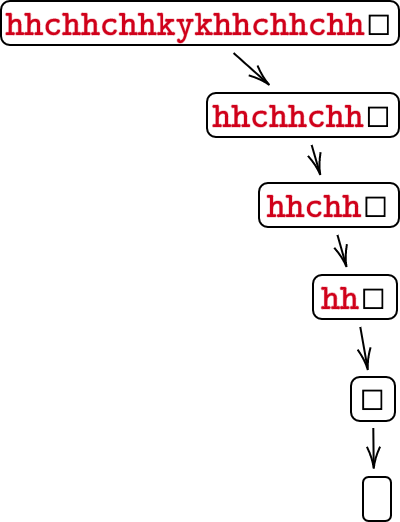
\includegraphics[scale=0.35]{assets/suffixLink.png}
\caption{Ilustrasi \textit{Suffix Link} untuk \textit{String} \texttt{hhchhchhkykhhchhchh}}
\end{figure}

\begin{lemma}
\label{levelNode}
Pada \textit{node} ke-$v$, setiap $edge[v][c] = u$ akan mengarah ke \textit{node} $u$ dengan $len[u] = len[v] + 2$. Secara trivial, \textit{node} selain \textit{root} akan memiliki tepat satu \textit{edge} yang masuk ke \textit{node} tersebut.
\end{lemma}

\begin{proposition}
Untuk \textit{string} $S$ sepanjang $n$, Eertree dari \textit{string} ini dapat dibuat secara \textit{online} dalam kompleksitas waktu terburuk $O(n \log |\sigma|)$.
\end{proposition}

\begin{proof}
Perhatikan bahwa akan dilakukan iterasi untuk setiap karakter untuk $S$ dari $1$ sampai $n$. Dalam iterasi ke-$i$, akan disimpan posisi penunjuk \textit{node} (\textit{pointer}) saat ini. Penunjuk \textit{node} akan menunjuk ke \textit{node} yang merepresentasikan \textit{substring} palindrom terpanjang yang berakhir pada indeks $i$.

Berdasarkan \hyperref[levelNode]{Lema 3.3}, setiap \textit{node} $v$ bisa kita anggap memiliki level atau tingkatan berdasarkan panjangnya, yaitu $len[v]$. Definisikan penunjuk saat ini merupakan $p$ untuk indeks $i$. Diketahui bahwa \textit{node} yang ditunjuk oleh $p$ memiliki panjang $len[p]$ dan merepresentasikan \textit{substring} palindrom $S[i - len[p] + 1, i]$.

Saat melakukan penambahan karakter baru $c = S[i + 1]$, maka akan dibandingkan apakah $S[i - len[p]] = c$. Bila tidak sama, maka kita dapat membandingkannya dengan \textit{suffix link} dari $p$, atau dibuat menjadi $p' := link[p]$. Proses ini tentunya menurunkan panjang dari $p$ untuk iterasi selanjutnya. Bila saat melakukan \textit{traversal} dan membandingkan $S[i - len[p]] = c$ bernilai benar. Akan ada dua kasus yang harus diobservasi.

\begin{itemize}
    \item Bila $edge[p][c]$ sudah ada, maka atur $p = edge[p][c]$. Tentunya, \textit{node} ini sudah ada sebelumnya, dan jumlah \textit{substring} palindrom berbeda tidak akan bertambah.
    \item Bila $edge[p][c]$ belum mengarah ke \textit{node} mana pun, maka ditemukan sebuah \textit{substring} palindrom baru yang belum pernah ada di dalam Eertree. Akan dibuat \textit{node} baru dengan indeks terkecil yang belum ada di dalam \textit{tree}, yang merepresentasikan \textit{substring} $cS[i - len[p] + 1, i]c = S[i - len[p], i + 1]$. Definisikan \textit{node} ini sebagai $u$, arahkan $edge[p][c] := u$, dan $len[u] = len[p] + 2$. Sekarang, akan dicari \textit{suffix link} dari \textit{node} $u$. \textit{Suffix link} dari \textit{node} ini merupakan \textit{suffix} palindrom kedua terpanjang yang berakhir pada indeks $i + 1$. Dalam mencarinya, dapat dilakukan \textit{traversal} terus menerus melanjutkan iterasi $p' = link[p]$, hingga ditemukan $p'$ sedemikian sehingga $S[i - len[p']] = c$.
\end{itemize}

Pencarian \textit{suffix link} tentu saja akan berhenti, dengan kasus basis saat $p = -1$, tentunya \textit{node} tersebut akan berakhir dengan sebuah \textit{substring} satu karakter $c$ dalam kasus terburuk pencariannya. Kompleksitas waktu dari algoritma penambahan karakter ini dapat dianalisis secara \textit{amortized}.

Meskipun \textit{traversal suffix link} terlihat dapat terjadi dalam $\Theta(n)$ dalam kasus terburuknya, secara keseluruhan dalam pembuatan \textit{tree} ini tidak akan mencapai $\Theta(n^2)$. Secara intuitif, misalkan terdapat dua \textit{pointer} atau penunjuk, $l$ dan $r$. $l$ menunjuk kepada batas kiri dari \textit{substring} palindrom terpanjang pada iterasi ke-$r$. Dalam setiap iterasinya, $r$ akan bertambah $1$ karena karakter baru akan ditambahkan. Saat melakukan \textit{traversal suffix link} untuk mencari nilai $p$ selanjutnya, penunjuk $l$ akan bertambah $1$ atau bergerak ke kanan, hingga berlaku $S[l - 1] = S[r + 1]$ dan $l$ akan bergerak ke kiri sebanyak satu kali setiap iterasinya. 

Perhatikan bahwa pergerakan ke kanan akan terjadi paling banyak $n$ kali secara keseluruhan, dan tepat $n$ kali ke kiri (tidak menutup kemungkinan terdapat sebuah iterasi yang membuat pergerakan ke kanan dilakukan sebanyak $r$ kali secara langsung). Secara total, pergerakan tersebut tidak akan bergerak lebih dari $2n$ kali. 

Selain mencari nilai $p$ selanjutnya, mencari \textit{suffix link} dari \textit{node} yang baru juga sama. Bisa direduksi menjadi kasus mencari \textit{suffix} palindrom kedua terpanjang yang ada. Simpan pula sebuah nilai $m$ yang menunjuk pada \textit{suffix} palindrom kedua terpanjang pada iterasi ke-$r$. Dengan argumen yang sama, pergerakan $m$ secara total tidak akan bergerak lebih dari $2n$ kali.

Faktor kompleksitas waktu $\log |\sigma|$ muncul saat mencari nilai dari $edge[v][c]$, untuk sembarang \textit{node} $v$ dan karakter $c$. Dengan struktur data \textit{hash}, atau \textit{array} sederhana, nilai indeks ini dapat dicari dalam kompleksitas waktu $O(1)$. Secara analisis, bisa digunakan struktur data \textit{Balanced Binary Search Tree} sederhana untuk himpunan $\sigma$ yang lebih banyak. Sehingga, kompleksitas waktu dalam membuat Eertree untuk \textit{string} $S$ dengan panjang $n$ ialah $O(n \log |\sigma|)$, dengan kompleksitas memori $O(n)$.
\end{proof}

\section{Implementasi dan Eksperimen}

Berikut ialah pseudocode dari bagian inisialisasi dari Eertree.

\SetKwComment{Comment}{// }{}
\begin{algorithm}
\DontPrintSemicolon
\caption{Melakukan inisialisasi pada Eertree}\label{alg:init}
$len[0] := -1$\Comment*[]{Indexing 0-based, 2 \textit{node} khusus}
$link[0] := 0$\;
$len[1] := 0$\;
$link[1] := 0$\;
$lastPointer := 0$\Comment*[]{lastPointer awalnya pada \textit{node} -1}
$n := 0$\Comment*[]{Panjang \textit{string} yang sudah diproses}
$size := 2$\Comment*[]{Ukuran Eertree}
\end{algorithm}

\textit{Pseudocode} dari bagian penambahan karakter $c$ pada Eertree saya cantumkan pula. Kompleksitas waktu yang diperlukan untuk bagian ini ialah $O(n)$. Secara total, dalam menambahkan $n$ karakter, dibutuhkan waktu $\Theta(n)$ saja.

\begin{algorithm}
\DontPrintSemicolon
\caption{Algoritma untuk melakukan \texttt{add}(c) pada Eertree}\label{alg:add}
\KwData{\\$c$ --- karakter yang ingin ditambahkan\\
$n$ --- panjang \textit{string} yang sudah dimasukkan ke Eertree\\
$lastPointer$ --- penunjuk \textit{node} setelah memasukkan karakter terakhir, yaitu $S[n]$\\
$S$ --- \textit{string} yang diproses\\
$edge[v][c]$ --- \textit{adjacency node} untuk \textit{node} $v$ terhadap setiap karakter $c \in \sigma$\\
$link[v]$ --- \textit{suffix link} dari node $v$\\
$len[v]$ --- panjang dari \textit{node} $v$\\
$size$ --- ukuran Eertree\\
}
\While{$n - len[lastPointer] - 1 < 0$ \onlyb{atau} $S[n - len[lastPointer] - 1] \ne c$}{
    \Comment*[l]{Mencari longest suffix palindrom terbaru}
    $lastPointer = link[lastPointer]$\;
}
\If{edge[lastPointer][c] \noSty{belum ada}}{
    \Comment*[l]{Membuat node baru}
    $newNode := size$\;
    $size := size + 1$\;
    $edge[lastPointer][c] := newNode$\;
    $len[newNode] = len[lastPointer] + 2$\;
    \eIf{len[newNode] = 1}{
        \Comment*[l]{Kasus saat panjang = 1}
        $link[lastPointer] := 1$\;
    }{
        \Comment*[l]{Mencari second best suffix palindrom}
        $secondBest := link[lastPointer]$\;
        \While{$S[n - len[secondBest] - 1] \ne c$}{
            $secondBest := link[secondBest]$\;
        }
        $link[newNode] := edge[secondBest][c]$\;
    }
}
$n := n + 1$\;
$lastPointer := edge[lastPointer][c]$\;
\end{algorithm}

Berikut ialah ilustrasi berjalannya algoritma saat memproses \textit{string} $\texttt{hckkcykokoky}$.

\begin{figure}[H]
\centering
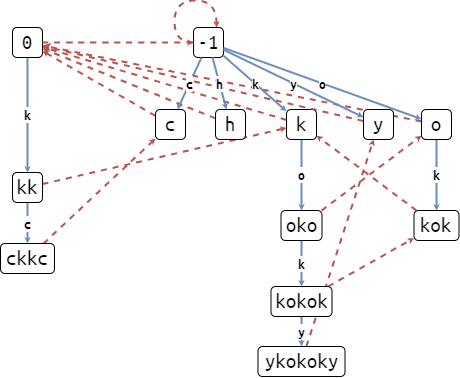
\includegraphics[scale=0.4]{assets/eertree.png}
\caption{Ilustrasi Eertree untuk \textit{String} \texttt{hckkcykokoky}}
\end{figure}

Pada mulanya hanya akan ada \textit{node} yang bertanda $0$ dan $-1$ sebagai \textit{root}. Garis putus-putus berwarna merah ditandai sebagai \textit{suffix link} dan garis biasa berwarna biru menandakan adanya \textit{edge} dari \textit{node} tersebut ke anak-anaknya, dengan huruf pada \textit{edge} merupakan karakter yang \textit{berkorespondensi} atas hubungan tersebut. \textit{Node} penunjuk saat ini akan menunjuk pada \textit{node} yang di-\textit{highlight} biru.

\begin{figure}[H]
\centering
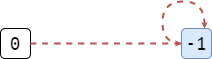
\includegraphics[scale=0.4]{assets/eer01.png}
\caption{Kondisi Eertree Setelah Inisialisasi}
\end{figure}

Pada awalnya \textit{node} akan penunjuk berada pada \textit{node} $-1$. Saat ditambahkan huruf $\texttt{h}$, akan dicek apakah \textit{suffix} dengan panjang $-1 + \textbf{2} = 1$ karakter, termasuk karakter yang baru ditambahkan ini merupakan palindrom. Secara trivial, jelas bahwa \textit{suffix} ini merupakan karakter. Untuk \textit{node} dengan panjang $1$, \textit{suffix link} secara khusus akan dihubungkan pada \textit{node} $0$. Begitu pula selanjutnya bila ditambahkan \textit{node-node} lain. Perhatikan bahwa pada saat \textit{traversal suffix link} pada \textit{node} $0$, akan dicek apakah \textit{suffix} palindrom dengan panjang $2$, (misal $\texttt{hh}$, $\texttt{cc}$, atau $\texttt{kk}$) merupakan palindrom. Tentunya dalam kasus ini pencocokan \textit{string} tidak berhasil, sehingga akan kembali ke \textit{suffix link}-nya, yaitu $-1$.

\begin{figure}[H]
\centering
\begin{subfigure}[b]{0.4\textwidth}
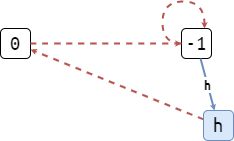
\includegraphics[scale=0.5]{assets/eer02.png}
\caption{$S[1, i] = \texttt{h}$}
\end{subfigure}
\begin{subfigure}[b]{0.4\textwidth}
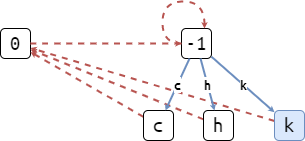
\includegraphics[scale=0.5]{assets/eer03.png}
\caption{$S[1, i] = \texttt{hck}$}
\end{subfigure}
\caption{Kondisi Eertree}
\end{figure}

Perhatikan bahwa saat penambahan karakter ke-$4$, terdapat \textit{suffix} palindrom $\texttt{kk}$ dengan panjang $2$, selanjutnya akan dibuat \textit{node} baru yang merepresentasikan \textit{substring} $\texttt{kk}$. Akan dicari \textit{suffix link} untuk \textit{node} baru ini. Dari $\texttt{k}$ akan menuju ke \textit{node} $0$ \textit{traversal suffix link}-nya, ditemukan \textit{suffix} palindrom dengan panjang $1$, yaitu $\texttt{k}$. Sehingga \textit{node} baru $\texttt{kk}$ yang dibuat akan dihubungkan ke $\texttt{k}$.

Pada saat penambahan karakter ke-$5$ kasusnya mirip. Awalnya \textit{traversal suffix link} akan dimulai dari $\texttt{k}$, akan dicek apakah terdapat \textit{node} $\texttt{ckc}$, yang bisa menjadi potensial arah \textit{suffix link} dari \textit{node} baru $\texttt{ckkc}$, ternyata tidak ada. Kemudian akan lanjut ke \textit{node} $0$, ditemukan \textit{node} $\texttt{c}$ sebagai \textit{suffix link} dari $\texttt{ckkc}$.

\begin{figure}[H]
\centering
\begin{subfigure}[b]{0.45\textwidth}
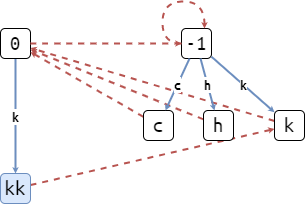
\includegraphics[scale=0.45]{assets/eer04.png}
\caption{$S[1, i] = \texttt{hckk}$}
\end{subfigure}
\begin{subfigure}[b]{0.45\textwidth}
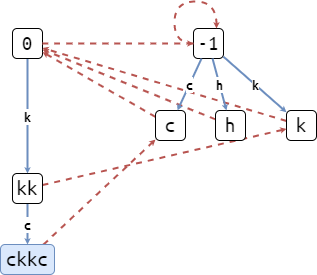
\includegraphics[scale=0.45]{assets/eer05.png}
\caption{$S[1, i] = \texttt{hckkc}$}
\end{subfigure}
\caption{Kondisi Eertree}
\end{figure}

\begin{figure}[H]
\centering
\begin{subfigure}[b]{0.45\textwidth}
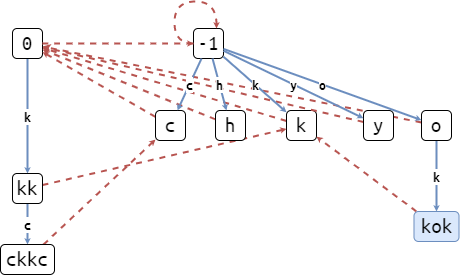
\includegraphics[scale=0.45]{assets/eer07.png}
\caption{$S[1, i] = \texttt{hckkcykok}$}
\end{subfigure}
\begin{subfigure}[b]{0.45\textwidth}
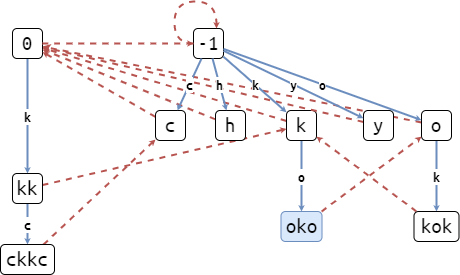
\includegraphics[scale=0.4]{assets/eer08.png}
\caption{$S[1, i] = \texttt{hckkcykoko}$}
\end{subfigure}
\caption{Kondisi Eertree}
\end{figure}

Proses yang sama dapat dilakukan saat penambahan \textit{string-string} selanjutnya, serupa dengan menangani \textit{string} dengan panjang genap. Selanjutnya perhatikan juga bahwa saat penambahan karakter $\texttt{k}$ pada \hyperref[eer9]{Gambar 7.a}. \textit{Suffix link} pada \textit{node} baru $\texttt{kokok}$ akan dihubungkan menuju \textit{node} \texttt{kok}, karena \textit{suffix link} kedua \textit{terpanjang}-nya merupakan \texttt{kok}.

\begin{figure}[H]
\label{eer9}
\centering
\begin{subfigure}[b]{0.45\textwidth}
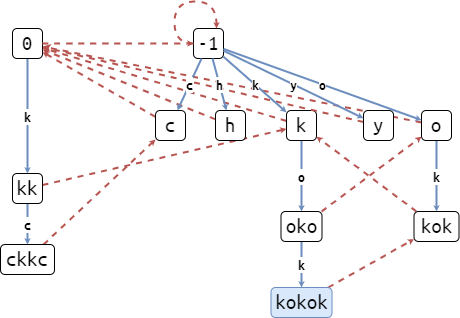
\includegraphics[scale=0.4]{assets/eer09.png}
\caption{$S[1, i] = \texttt{hckkcykokok}$}
\end{subfigure}
\begin{subfigure}[b]{0.45\textwidth}
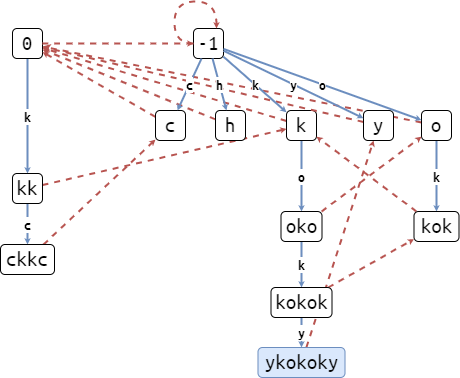
\includegraphics[scale=0.45]{assets/eer10.png}
\caption{$S[1, i] = \texttt{hckkcykokoky}$}
\end{subfigure}
\caption{Kondisi Eertree}
\end{figure}

Selanjutnya, akan dicoba implementasi Eertree tersebut pada C++. Menggunakan kode yang sama, dilakukan percobaan $5$ kali untuk masing-masing \textit{string} $S$ yang terdiri dari huruf latin kecil acak (\texttt{a} - \texttt{z}) sepanjang $n$ dan dihitung rata-rata dari penggunaan waktunya hanya dalam pembuatan Eertree untuk \textit{string} tersebut. Program juga dijalankan pada komputer penulis, sehingga perbedaan waktu pada mesin yang berbeda tidak dapat dihindari. Eksperimen ini dilakukan hanya untuk mengetahui laju peningkatan waktu komputasi.

\begin{table}[h]
    \centering
    \begin{tabular}{|c|c|c|c|c|c|c|}
    \hline
        $n$ & $10^3$ & $10^4$ & $10^5$ & $10^6$ & $10^7$ & $10^8$\\
    \hline
        $t$ (aproksimasi dalam ms) & $0.002 $ & $0.006$ & $1.4126$ & $10.9952$ & $92.2064$ & $1043.3976$\\
    \hline
    \end{tabular}
    \caption{Waktu Pembuatan Eertree untuk \textit{String} $S$ Sepanjang $n$ Tertentu}
\end{table}

Untuk $n = 10^8$, waktu yang diperlukan ialah sekitar $1$ detik. Bila diperhatikan, disini perkembangan waktunya linear. Hal ini disebabkan karena $|\sigma|$ yang berjumlah tetap, yaitu $26$. Alokasi memori disediakan oleh sistem operasi menggunakan array. Sehingga bila dihitung menggunakan ram model, kompleksitas waktu yang diperlukan ialah $\Theta(n)$. Dari eksperimen dan pembuktian, dapat terlihat bahwa kecepatan fungsi waktu tumbuh memang bersifat linear pula. Namun berbeda dengan kompleksitas memorinya. Dilakukan eksperimen pula untuk banyaknya verteks rata-rata dengan batasan yang sama. Dilakukan $5$ kali percobaan, dan dihitung rata-ratanya.

\begin{table}[h]
    \centering
    \begin{tabular}{|c|c|c|c|c|c|c|}
    \hline
        $n$ & $10^3$ & $10^4$ & $10^5$ & $10^6$ & $10^7$ & $10^8$\\
    \hline
    \hline
Percobaan $1$ & 77 & 381 & 996 & 2850 & 12540 & 29929 \\ \hline
Percobaan $2$ & 96 & 345 & 1042 & 2913 & 12591 & 30001 \\ \hline
Percobaan $3$ & 72 & 370 & 1019 & 2813 & 12577 & 30023 \\ \hline
Percobaan $4$ & 90 & 383 & 1003 & 2867 & 12595 & 29923 \\ \hline
Percobaan $5$ & 71 & 390 & 992 & 2839 & 12670 & 30062 \\ \hline
Rata-rata & 81.2 & 373.8 & 1010.4 & 2856.4 & 12594.6 & 29987.6 \\ \hline
    \end{tabular}
    \caption{Banyaknya Verteks Eertree untuk \textit{String} $S$ Sepanjang $n$ Tertentu}
\end{table}

\begin{figure}[H]
\centering
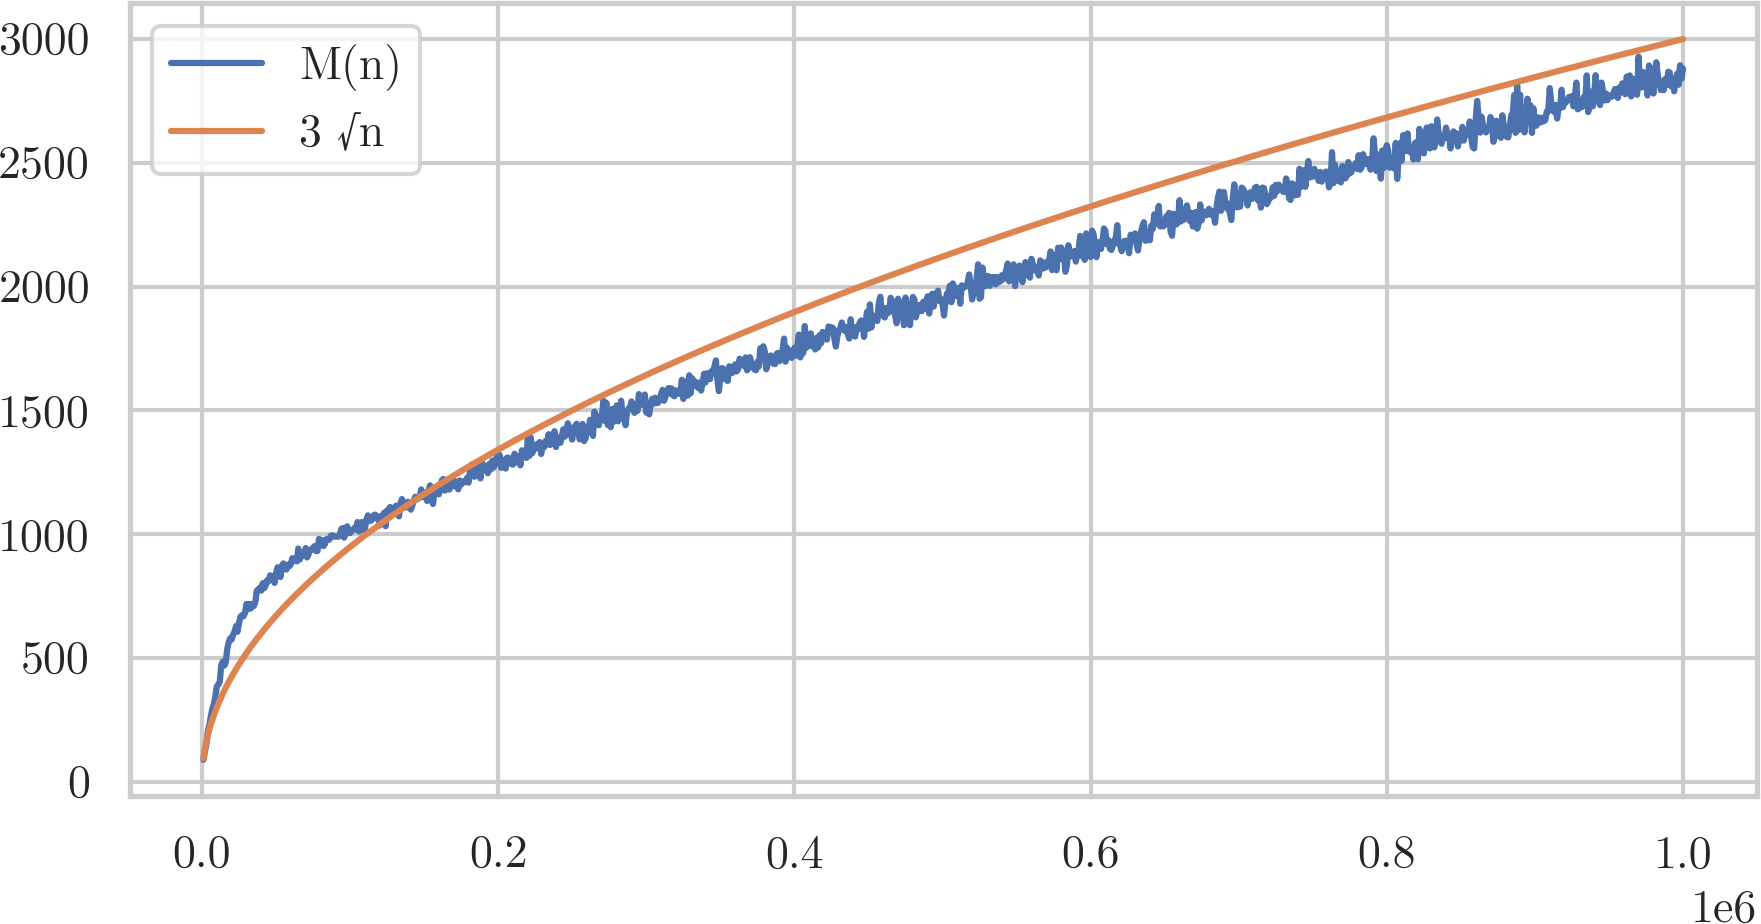
\includegraphics[scale=1]{assets/memory.png}
\caption{Nilai \textit{String} $S$ Acak Sepanjang $n$ terhadap Banyaknya Verteks pada Eertree}
\end{figure}

Berdasarkan eksperimen yang saya lakukan dan pembuktian yang sudah pernah dilakukan juga, diketahui bahwa kompleksitas memori rata-rata yang dibutuhkan Eertree untuk \textit{string} $S$ acak sepanjang $n$ ialah $\Theta(\sqrt{n|\sigma|})$ \cite{rubinchik2016number}.

\section{Aplikasi dan Variasi Eertree}

\subsection{Mencari Kemunculan Jumlah Setiap Substring Palindrom}

Perhatikan bahwa saat menambahkan satu karakter $c$, kemunculan \textit{substring-substring} palindrom (tidak harus berbeda) akan bertambah. \textit{Substring-substring} ini merupakan semua \textit{substring} dari root $0$ atau $-1$ hingga ke \textit{node} saat ini. Bila kita perhatikan kembali \hyperref[eer9]{Gambar 7.a}. Saat menambahkan karakter $k$, maka akan bertambah kemunculan dari $kokok$, $kok$, dan $k$. Untuk menghitung ada berapa banyak kemunculan masing-masing palindrom ini, bisa ditambahkan sebuah nilai $occ[lastPointer]$ untuk setiap \textit{node} yang dikunjungi oleh $lastPointer$ sembari memasukkan setiap karakter. Setelah pembuatan Eertree selesai, iterasi dapat dilakukan untuk indeks \textit{node} yang terbesar hingga yang terkecil, dengan melakukan penambahan seperti \textit{suffix sum}, dengan kata lain $occ[link[v]] := occ[link[v]] + occ[v]$. Setelah komputasi ini, maka akan didapatkan kemunculan \textit{substring} tersebut untuk setiap \textit{node} $v$.

\begin{algorithm}
\DontPrintSemicolon
\caption{Menghitung kemunculan jumlah setiap \textit{substring}}\label{alg:occ_sub}
\For{i := 1 \KwTo n}{
$add(S[i])$\;
$occ[lastPointer] := occ[lastPointer] + 1$\;
}

\For{i := size \KwTo 1}{
$occ[link[i]] := occ[link[i]] + occ[i]$\;
}
\end{algorithm}

\subsection{Mencari Banyaknya Substring Palindrom yang Diakhiri pada Indeks Tertentu}

\begin{lemma}
\textit{Suffix link} membentuk tree dengan root pada $-1$ dan $0$.
\end{lemma}

\begin{proof}

Perhatikan bahwa setiap \textit{node} memiliki tepat satu \textit{suffix link} dengan asumsi bahwa \textit{suffix link} yang menghubungkan $-1$ dengan dirinya sendiri tidak dihitung, maka tepat terdapat $n + 1$ \textit{edge} dan $n + 2$ \textit{node} yang terbentuk dari \textit{tree} \textit{suffix link} ini untuk sebuah \textit{string} $S$ sepanjang $n$. Karena \textit{suffix link} sebuah \textit{node} $v$, yaitu $link[v] = u$ hanya menghubungkan \textit{proper suffix} palindrom dan berlaku $len[u] < len[v]$. Maka dipastikan tidak ada \textit{cycle} yang terbentuk pada graf ini. Sehingga graf ini merupakan \textit{tree}.
\end{proof}

Perhatikan bahwa banyaknya \textit{string} yang diakhiri pada suatu indeks $R$ ialah panjang atau kedalaman \textit{node} saat ini bila dilihat dari \textit{tree} yang terbentuk dari \textit{suffix link}-nya. Sehingga, dapat dilakukan \textit{Breadth First Search} atau \textit{Depth First Search} dari \textit{node} $-1$ hingga ke \textit{node} $n$. Selanjutnya, setelah melakukan $add(c)$ untuk setiap indeks $i$, perlu disimpan $idx[i] := lastPointer$ nilai penunjuk \textit{node} setelah memasukkan karakter ke-$i$, yaitu $S[i]$. 

Kemudian simpan pula nilai $occ[v]$ untuk setiap \textit{node} pada Eertree yang awalnya nilai satu. Setelah dilakukan \textit{Depth First Search} yang serupa dengan \textit{prefix sum} melalui \textit{tree suffix link}-nya, atau $occ[v] := occ[v] + occ[link[v]]$. Banyaknya \textit{substring} palindrom yang diakhiri pada indeks $R$ ialah $occ[idx[R]]$. Untuk mendapatkan banyaknya \textit{substring} palindrom yang dimulai pada suatu indeks $L$, dapat dibuat sebuah Eertree untuk kebalikan atau \textit{reverse} dari \textit{string} $S$. Selanjutnya lakukan komputasi yang serupa. Banyaknya \textit{substring} palindrom yang dimulai pada suatu indeks $L$ ialah $occ[idx[n - L + 1]]$.

\begin{algorithm}
\DontPrintSemicolon
\caption{Menghitung banyak \textit{substring} yang diakhiri pada indeks $R$}\label{alg:end_R}
\For{i := 1 \KwTo n}{
$add(S[i])$\;
$idx[i] := lastPointer$\;
}

\For{i := 2 \KwTo size}{
$occ[i] := 1$\;
$occ[i] := occ[i] + occ[link[i]]$\;
}

\onlyb{return} $occ[idx[R]]$
\end{algorithm}

% \begin{algorithm}
% \DontPrintSemicolon
% \caption{Menghitung banyak substring yang diawali pada indeks $L$}\label{alg:start_L}
% $S[i] = reverse(S[i])$\;

% \For{i := 1 \KwTo n}{
% $add(S[i])$\;
% $idx[i] := lastPointer$\;
% }

% \For{i := 2 \KwTo size}{
% $occ[i] := 1$\;
% $occ[i] := occ[i] + occ[link[i]]$\;
% }

% \onlyb{return} $occ[idx[n - L + 1]]$
% \end{algorithm}

\subsection{Lebih Dari Satu String}

Eertree tidak hanya bisa mewakili satu \textit{string} saja. Ada variasi lain dari Eertree yang bisa dimanfaatkan. Eertree yang dibentuk dari beberapa \textit{string} dapat dibuat dengan membuat Eertree untuk \textit{string} pertama, mengembalikan penunjuk \textit{node} saat ini ke posisi \textit{node} awal, yaitu $-1$. Kemudian lakukan operasi pembuatan Eertree kembali untuk \textit{string} kedua, dengan tidak mengabaikan \textit{node-node}, \textit{edges}, dan \textit{suffix link} yang sudah ada pada \textit{Eertree} saat ini. Begitu seterusnya hingga setiap \textit{string} selesai diproses. Pada umumnya, untuk setiap \textit{node}, akan disimpan pula suatu penanda apakah \textit{node} ini ada pada \textit{string} ke-$i$. Sehingga, setiap \textit{node} akan menyimpan nilai tambahan $exist[v][i]$ yang menandakan bahwa \textit{node} ke-$v$ terkandung pada saat membuat \textit{string} ke-$i$.

\subsection{Operasi Penghapusan}

Selain operasi \texttt{add(c)}, terdapat variasi Eertree yang mendukung operasi \texttt{pop()}. Salah satu yang menjadi hambatan dalam mendukung operasi ini ialah operasi \texttt{add(c)} yang memiliki kompleksitas waktu $O(n)$. Sehingga operasi \texttt{pop()} dan \texttt{add(c)} terus menerus pada kasus terburuk pencarian \textit{suffix link} terpanjang-nya, bisa menyebabkan kompleksitas $O(nq)$. Untuk $q$ banyaknya operasi $\texttt{pop}$ yang dilakukan. Salah satu kasusnya ialah:

\[\underbrace{\texttt{add(h)},\texttt{add(h)}, \dots, \texttt{add(h)},\texttt{add(h)}}_\text{Sebanyak $n$ kali}\underbrace{\texttt{add(o)},\texttt{pop()}, \dots, \texttt{add(o)},\texttt{pop()}}_\text{Sebanyak $q$ kali}\]

Setiap kali operasi \texttt{add(o)} dilakukan, pencarian \textit{suffix link} dari \texttt{o} akan terus menerus dilakukan dengan \textit{suffix} palindrom sebagai berikut.

\[\underbrace{hhhh\dots hhhh}_\text{Sepanjang n} \rightarrow \underbrace{hhhh\dots hhh}_\text{Sepanjang n - 1} \rightarrow \cdots \rightarrow hhh \rightarrow hh \rightarrow h \rightarrow \text{Node } 0 \rightarrow \text{Node } {-1}\]

Terdapat beberapa alternatif dalam mempercepat proses \texttt{add(c)} ini, oleh penemu struktur data ini, dinamakan \textit{quick link} dan \textit{direct link}.

\subsubsection{Quick Link}

Quick link pada dasarnya mempercepat proses saat ada beberapa karakter yang sama dalam sebuah rantai \textit{suffix link}. Saat \textit{traversal suffix link}, akan dilakukan perbandingan-perbandingan karakter sebelum \textit{substring} dengan karakter baru yang akan ditambahkan untuk setiap \textit{suffix} palindrom.

Pada \textit{suffix} palindrom seperti \texttt{hhh\dots hhh} atau  \texttt{haha\dots haha}, huruf \texttt{h} akan dibandingkan berulang-ulang kali dengan kompleksitas panjang $\Theta(n)$ dengan $n$ panjang \textit{substring} tersebut. Secara intuitif, perhatikan bahwa untuk dua huruf berbeda dalam sebuah rantai \textit{suffix link} bisa terbuat, maka panjang palindrom harus setidaknya dua kalinya. Misalnya kita akan mencoba secara \textit{greedy} untuk membuat sebuah rantai \textit{suffix} palindrom terpendek sehingga saat tidak ada dua huruf berurutan yang sama akan dibandingkan dalam \textit{traversal}-nya. Tanpa mengurangi sifat umum, anggap dua huruf di sini \texttt{a} dan \texttt{h}.

$$\texttt{\textbf{h}} \rightarrow \texttt{\textbf{a}h} \rightarrow \texttt{\textbf{h}hah} \rightarrow \texttt{\textbf{a}hahhah} \rightarrow \texttt{\textbf{h}hahhahahhah} \rightarrow \dots$$

Pembuktian lebih formal dan lengkapnya dapat dilihat pada jurnal \cite{kosolobov2015mathrmpalk}. Karena adanya sifat ini, maka \textit{quick link} dapat mempercepat \textit{traversal suffix link} dan membuat kompleksitasnya hanya menjadi $O(\log n)$ untuk setiap operasi \texttt{add(c)}. Untuk tambahan memori sendiri hanya perlu $\Theta(1)$ untuk setiap \textit{node}-nya. \textit{Implementasi}-nya sederhana, cukup menambahkan sebuah variabel baru $quickLink[v] = u$ yang menandakan $u$ adalah \textit{node} pertama dalam rantai \textit{suffix link} yang karakter ke $S[i - len[u]]$ nya tidak sama dengan $S[i - len[v]]$.

\subsubsection{Direct Link dengan Naive Array}

Berbeda dengan \textit{quick link}, sesuai namanya, akan disimpan sebuah \textit{link} yang menghubungkan ke \textit{suffix} palindrom dengan karakter yang langsung sama dengan karakter yang dibandingkan. Definisikan sebuah variabel baru, misalnya $u = direct[v][c]$ yang merupakan \textit{suffix link direct} ke \textit{node} yang memiliki karakter $S[i - len[u]] = c$. Perhatikan bahwa kini kompleksitas waktunya menjadi $\Theta(\log |\sigma|)$ dengan asumsi \textit{direct link} disimpan menggunakan suatu \textit{Balanced Binary Search Tree}, dan kompleksitas memorinya akan bertambah sebanyak $\Theta(|\sigma|)$ untuk setiap \textit{node}-nya.

Namun perhatikan bahwa biasanya banyak karakter dalam aplikasi sehari-hari tidak banyak, hanya $26$ pada umumnya, sehingga kompleksitas waktu dan memori tambahan untuk setiap \textit{node}-nya bisa dianggap konstan.

\subsubsection{Direct Link dengan Persistent Edges}

Untuk mempercepat implementasi \textit{direct link} yang sebelumnya, kita dapat menggunakan suatu struktur data persisten. Dalam kasus ini, yang paling mudah diimplementasi ialah Persistent Segment Tree. Untuk intuisinya, anggap terdapat sebuah \textit{segment tree} untuk setiap \textit{node}-nya. Pada dasarnya sebuah \textit{segment tree} pada leaf ke-$c$ akan menyimpan \textit{direct link} ke-$c$ untuk suatu \textit{node} $v$. Kemudian, bila ditambahkan modifikasi persisten, kurang lebih \textit{segment tree}-nya akan berbentuk sebagai berikut.

\begin{figure}[H]
\centering
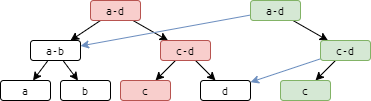
\includegraphics[scale=0.8]{assets/persistent.png}
\caption{Ilustrasi Persistent Segment Tree}
\end{figure}

Perhatikan bahwa \textit{tree} pada sebelah kiri istilahnya menunjukkan versi lama, dan pada saat melakukan \textit{insertion} pada \textit{segment tree}, akan dilakukan tambal sulam dan dibuat \textit{node-node} baru sebanyak $\Theta(\log n)$ untuk $n$ ukuran \textit{segment tree}, atau setara dengan kedalamannya. Perhatikan bahwa sekarang hanya perlu disimpan \textit{root} dari setiap versi, dan bisa diakses nilai-nilai dari setiap versinya. Sama halnya dalam kasus \textit{direct link} ini, setiap versi diibaratkan sebagai suatu \textit{node} $v$ baru. Setiap kali ada \textit{node} $v$ baru yang karakternya berbeda dengan rantai sebelumnya, maka bisa ditambahkan suatu tambal sulam baru.

Kompleksitas memori \textit{direct link} yang sebelumnya harus menyimpan nilai-nilai lainnya secara naif kini bisa turun. kompleksitas waktunya menjadi $O(\log |\sigma|)$ untuk operasi \texttt{add(c)} dan kompleksitas memorinya menjadi $O(\log |\sigma|)$ pula. Untuk lebih ketatnya, perhatikan bahwa bila karakter dalam rantai sama, maka tidak perlu dilakukan \textit{insertion} pada \textit{persistent segment tree}, dan berdasarkan bukti yang sudah dipaparkan sebelumnya, kompleksitas rantai \textit{quick link} paling panjang hanya $O(\log n)$, maka kompleksitas memorinya ialah $O(\min(\log |\sigma|, \log(\log n)))$.

\newpage
\nocite{*}
\bibliographystyle{apalike}
\bibliography{bibliography.bib}
\pagenumbering{gobble}


\newpage
\section*{Lampiran}
\newenvironment{code}{\captionsetup{type=listing}}{}
\SetupFloatingEnvironment{listing}{name=Kode Sumber}

\begin{code}
\captionof{listing}{Eertree}
\label{code:eertree-code}
\begin{minted}[
frame=lines,
framesep=2mm,
baselinestretch=1.2,
bgcolor=LightGray,
fontsize=\footnotesize,
linenos
]{cpp}
#include <bits/stdc++.h>
using namespace std;
using namespace std::chrono;
#define sz(x) (int)(x).size()

struct EerTree {
  struct Node {
    int next[26];
    int suffixLink;
    int length;
    Node() {
      memset(next, 0, sizeof(next));
      suffixLink = length = 0;
    }
  };
  string s;
  int n, lastPointer, lastIndex;
  vector <Node> tree;
  EerTree(const string &_s) {
    s = _s; tree.resize(3); init();
    for (int i = 0; i < sz(s); i++) {
      addChar(s[i]);
    }
  }
  EerTree(int _n) {
    s = ""; tree.resize(3); init();
  }
  void append(char ch) {
    s += ch; assert(sz(tree) > sz(s));
    addChar(s.back());
  }
  void init() {
    tree[0].suffixLink = 0;
    tree[0].length = -1;
    tree[1].suffixLink = 0;
    tree[1].length = 0;
    lastPointer = n = 0;
    lastIndex = 1;
  }
  void addChar(char ch) {
    int let = ch - 'a';
    while (n - tree[lastPointer].length - 1 < 0 || s[n - tree[lastPointer].length - 1] != ch)
      lastPointer = tree[lastPointer].suffixLink;
    if (!tree[lastPointer].next[let]) {
      tree[lastPointer].next[let] = ++lastIndex;
      if(lastIndex >= sz(tree)) tree.push_back(Node());
      tree[lastIndex].length = tree[lastPointer].length + 2;
      if (tree[lastIndex].length == 1) tree[lastIndex].suffixLink = 1;
      else {
        int ancestor = tree[lastPointer].suffixLink;
        while (s[n - tree[ancestor].length - 1] != ch) ancestor = tree[ancestor].suffixLink;
        tree[lastIndex].suffixLink = tree[ancestor].next[let];
      }
    }
    lastPointer = tree[lastPointer].next[let];
    n++;
  }
};

int main() {
  cin.tie(0)->sync_with_stdio(0);
  cin.exceptions(cin.failbit);
  string s; cin >> s;
  auto start = high_resolution_clock::now();
  EerTree solve(s);
  auto stop = high_resolution_clock::now();
  auto duration = duration_cast<microseconds>(stop - start);
  // cout << duration.count() << endl;
  cout << solve.lastIndex - 1 << endl;
}
\end{minted}
\end{code}

\begin{code}
\captionof{listing}{Kode Plot Kompleksitas Memori}
\label{code:plotting-code}
\begin{minted}[
frame=lines,
framesep=2mm,
baselinestretch=1.2,
bgcolor=LightGray,
fontsize=\footnotesize,
linenos
]{python}
import numpy as np
import seaborn as sns
import matplotlib.pyplot as plt
plt.figure(figsize=(7, 3.5))
sns.set_style(style='whitegrid')
sns.set_style({'font.family': 'CMU Serif'})
sns.lineplot(x = X, y = Y)
sns.lineplot(x = X, y = 3 * np.sqrt(X))
plt.legend(labels=["M(n)", "3\u221An"])
plt.savefig('memory.png', dpi = 300)
plt.show()
\end{minted}
\end{code}

\begin{code}
\captionof{listing}{Kode Generator \textit{String} Acak}
\label{code:string-gen-code}
\begin{minted}[
frame=lines,
framesep=2mm,
baselinestretch=1.2,
bgcolor=LightGray,
fontsize=\footnotesize,
linenos
]{cpp}
#include <bits/stdc++.h>
using namespace std;
mt19937 rng(chrono::steady_clock::now().time_since_epoch().count());

int getRange(int a, int b){
   int ran = b-a+1;
   return (rng()%ran)+a;
}

int main(){
  int n; cin >> n;
  for(int i = 1;i <= n;i++){
    cout << (char)(getRange(0, 25) + 'a'); 
  }
  cout << endl;
}
\end{minted}
\end{code}

\begin{figure}[H]
\centering
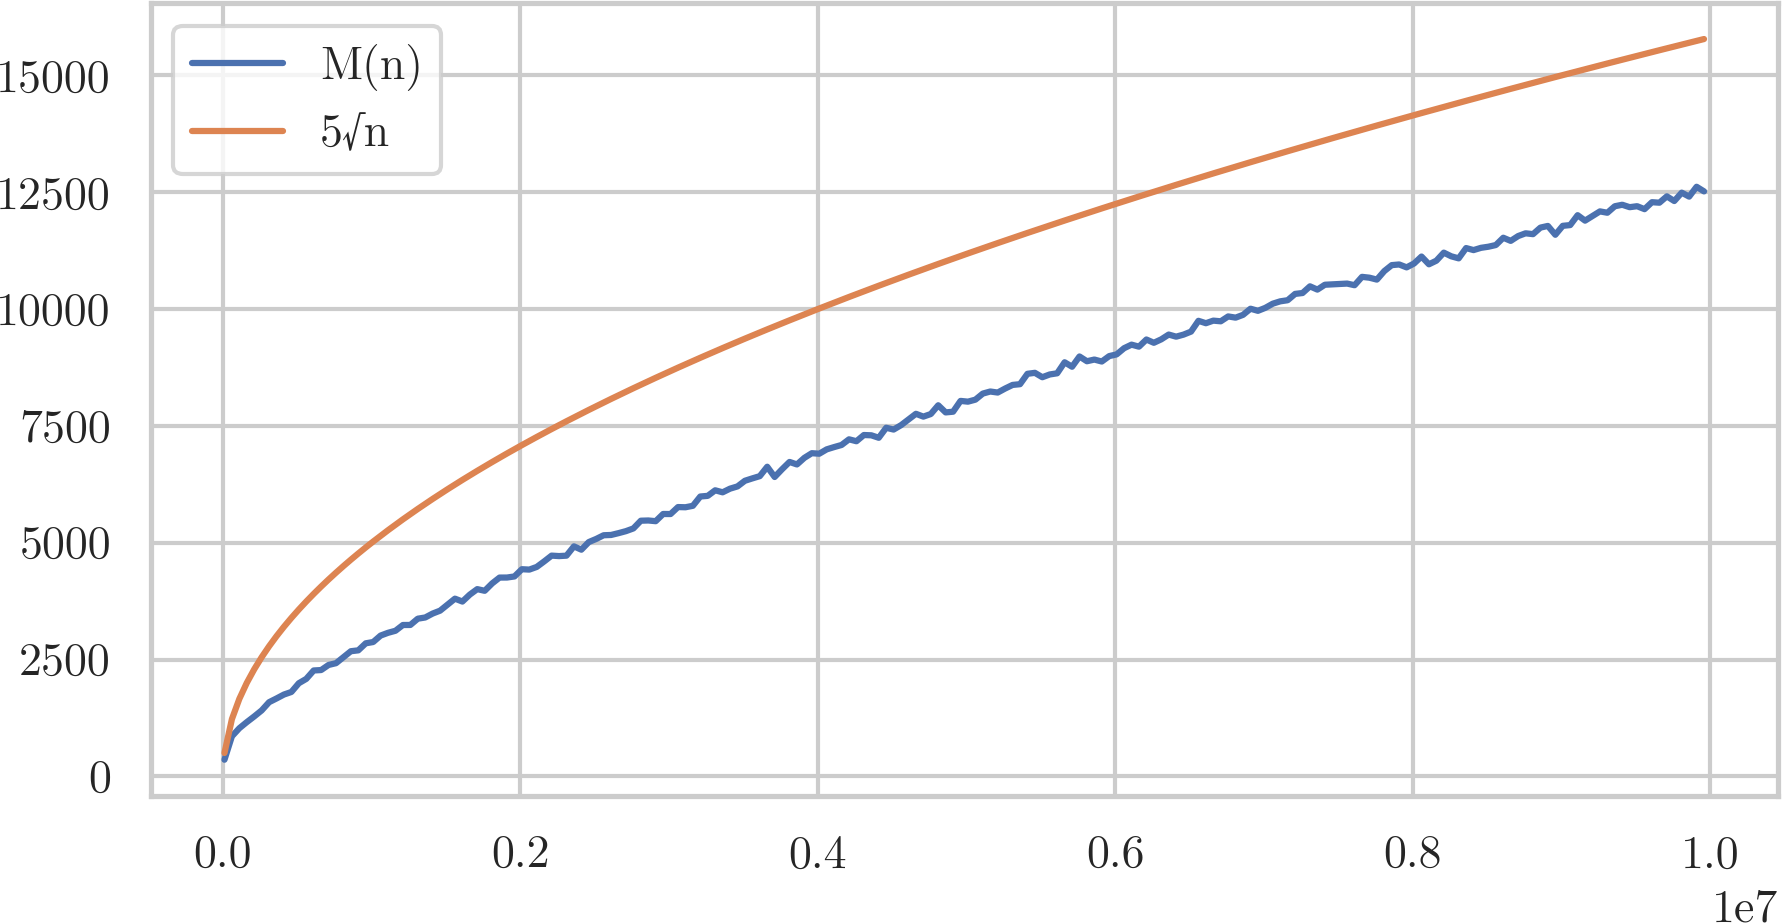
\includegraphics[scale=1]{assets/memory2.png}
\caption{Nilai \textit{String} $S$ Acak Sepanjang $n$ terhadap Banyaknya Verteks pada Eertree}
\end{figure}

\end{document}